\documentclass[tikz,border=2pt]{standalone}
\usepackage{amsmath,amssymb}
\usepackage{pgfplots}
\pgfplotsset{compat=1.18}
\usetikzlibrary{arrows.meta}

\begin{document}
% The directional derivative at x0 along v is the rate of change of f when moving from x0 in
% the direction v; for a differentiable f it equals the dot product ∇f(x0)·v.
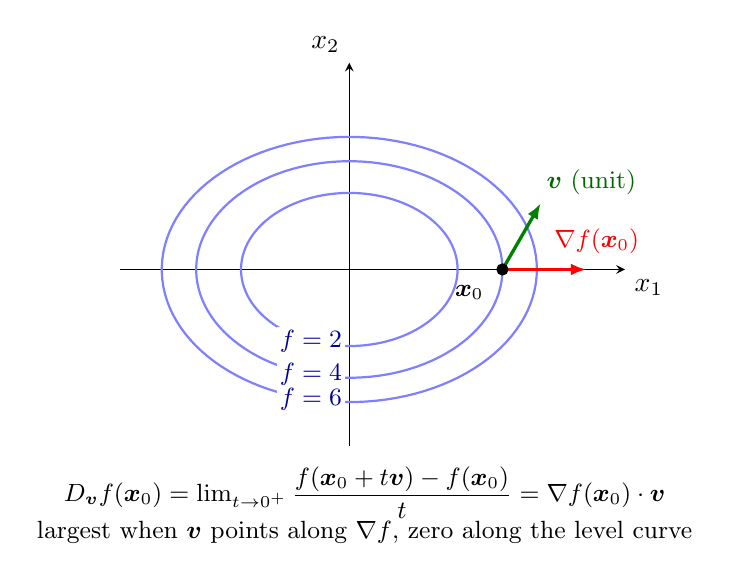
\begin{tikzpicture}
	\begin{axis}[
		axis lines=middle, axis equal image,
		xmin=-3.0, xmax=3.6, ymin=-2.3, ymax=2.7,
		xtick=\empty, ytick=\empty,
		xlabel={$x_1$}, ylabel={$x_2$},
		xlabel style={below right}, ylabel style={above left},
		clip=false, width=8cm
		]
		\foreach \c in {1,2,3} {
			\addplot[blue!50, thick, domain=0:360, samples=120] ({sqrt(\c*2)*cos(x)}, {sqrt(\c)*sin(x)});
		}
		\node[blue!60!black, font=\small, fill=white, inner sep=1pt] at (axis cs:-0.5,-0.935) {$f=2$};
		\node[blue!60!black, font=\small, fill=white, inner sep=1pt] at (axis cs:-0.5,-1.369) {$f=4$};
		\node[blue!60!black, font=\small, fill=white, inner sep=1pt] at (axis cs:-0.5,-1.696) {$f=6$};
		% x0 = (2,0) on f=4; grad = (4,0) scaled; v = unit vector at 60 degrees
		\addplot[only marks, mark=*, black] coordinates {(2,0)};
		\node[anchor=north east, font=\small] at (axis cs:1.88,-0.08) {$\boldsymbol{x}_0$};
		\draw[-{Latex[length=2mm]}, red, very thick] (axis cs:2,0) -- (axis cs:3.1,0);
		\node[red, anchor=south west, font=\small] at (axis cs:2.55,0.08) {$\nabla f(\boldsymbol{x}_0)$};
		\draw[-{Latex[length=2mm]}, green!50!black, very thick] (axis cs:2,0) -- (axis cs:2.5,0.866);
		\node[green!40!black, anchor=south west, font=\small] at (axis cs:2.45,0.85) {$\boldsymbol{v}$ (unit)};
		\node[anchor=north, font=\small, align=center] at (axis cs:0.2,-2.45) {$D_{\boldsymbol{v}}f(\boldsymbol{x}_0)=\lim_{t\to0^+}\dfrac{f(\boldsymbol{x}_0+t\boldsymbol{v})-f(\boldsymbol{x}_0)}{t}=\nabla f(\boldsymbol{x}_0)\cdot\boldsymbol{v}$\\ largest when $\boldsymbol{v}$ points along $\nabla f$, zero along the level curve};
	\end{axis}
\end{tikzpicture}
\end{document}
